\section{目的}
依 Lab 6（PDF 24--25 頁）比較實際 MOS 輸入負載與固定電容等效，檢查講義四組 8/16/24/32 fF 近似在本次模型是否成立。

\section{Spec 對照}
\begin{longtable}{p{0.31\linewidth}p{0.29\linewidth}p{0.31\linewidth}}
\toprule
講義要求（PDF頁） & 實作 & 驗證與界線 \\\midrule
步驟 1：表 6.1 四個案例（24--25） & 01\_gate\_load：NL=1--4 & 四例全部模擬 \\
比較 MOS 與固定電容波形／延遲（25） & 每個 MLOAD 對應 8 fF & 差異已量化，未宣稱近似相等 \\
\bottomrule
\end{longtable}


\section{電路與設計推導}
兩條路徑的驅動反相器相同：$W_n=0.6\,\mu$m、$W_p=1.8\,\mu$m、$L=0.25\,\mu$m。MOS 負載各為兩倍寬度 $1.2/3.6\,\mu$m；NL 個負載並接在同一驅動輸出，使用 MOS multiplicity 表示相同並聯單元，其輸出仍可切換。原始 case a 使用單倍負載、case b 將負載串接，與講義不同；已改成正確的兩倍、並聯負載。

手算 $C_g\approx C_{ox}(W_n+W_p)L$，$C_{ox}=\epsilon_{ox}/t_{ox}$。講義 $t_{ox}=5.4$ nm 對應每負載約 7.87 fF，只屬原模型；本次加密模型沒有可查驗的 $t_{ox}$，不冒用該數字。講義 W/L 的文字標示顛倒，本文採 W 為寬、L 為長。

\section{模擬設定}
本次為使用另行提供模型的教學改寫，電源為 1.0 V、溫度為 $25\,^{\circ}\mathrm C$。保留講義指定的拓樸、負載及比較尺寸；原講義的 2.5 V 製程結果不是本次模型的驗收數值。1 V 僅是模擬條件，不能視為模型的安全額定。所有 MOS 的 Bulk 明確接至相應電源軌。

HSPICE S-2021.09 使用 RUNLVL=6；保存波形、列印資料及原生量測。圖表由本次數據重繪；CSV 保存於各 Lab 的 results。完成模擬表示求解成功，並不代表製程可靠度已驗證。加密模型仍有被抑制的警告；既有診斷未取得可判讀的進一步內容，因此不宣稱警告無害或全部模型限制已滿足。

輸入 0.1 ns 邊緣、5 ns 週期；暫態 10 ns，列印 1 ps。每條路徑量測輸出 10--90\% 邊緣及輸入輸出 50\% 傳播延遲。

\section{結果與規格檢查}
四例求解與量測皆成功。下表單位 ps，MOS/C 分別指實際負載／固定電容。
\begin{center}\small
\begin{tabular}{llllll}
\toprule
NL & $C$ (fF) & $t_{pHL,MOS}$ & $t_{pHL,C}$ & $t_{pLH,MOS}$ & $t_{pLH,C}$ \\
\midrule
1 & 8 & 76.80 & 63.82 & 139.95 & 88.76 \\
2 & 16 & 112.89 & 85.88 & 241.42 & 127.05 \\
3 & 24 & 148.64 & 107.34 & 339.83 & 164.48 \\
4 & 32 & 184.10 & 128.38 & 439.90 & 201.64 \\
\bottomrule
\end{tabular}
\end{center}

\begin{figure}[htbp]
\centering
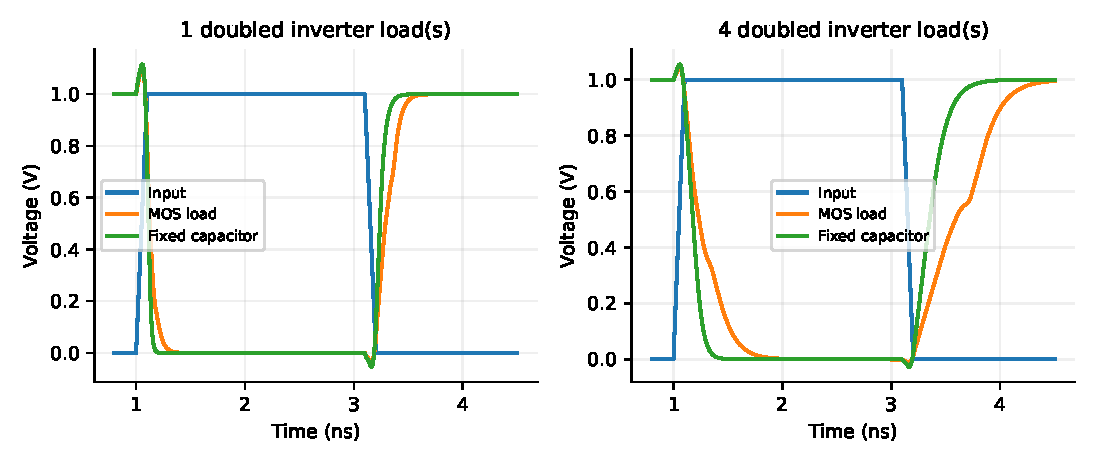
\includegraphics[width=\linewidth]{figures/gate_load_waveforms.pdf}
\caption{一個與四個負載的波形比較；由本次 HSPICE 數據重繪。}
\end{figure}

\begin{figure}[htbp]
\centering
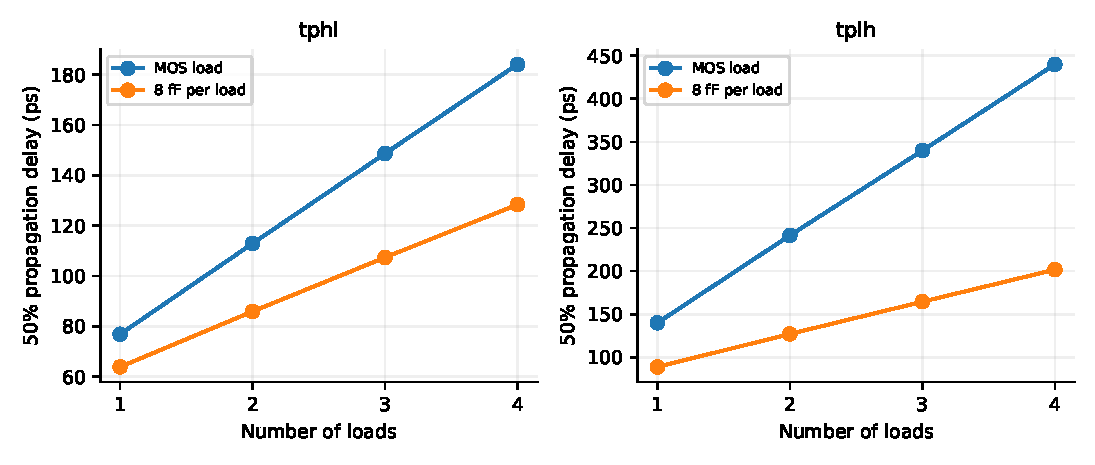
\includegraphics[width=\linewidth]{figures/gate_load_delays.pdf}
\caption{兩種負載的傳播延遲；由本次 HSPICE 數據重繪。}
\end{figure}


\section{討論}
MOS 負載在四個案例中皆比講義固定電容慢，尤其充電延遲：NL=4 為 439.90 ps，相較 32 fF 的 201.64 ps。差異來自本次模型的閘極電容、重疊／Miller 耦合及移動的負載輸出，不能只以單一 $C_{ox}WL$ 代表所有狀態。講義「近似相等」在本次條件下未重現，這是明確的模型移轉差異，不是省略實驗。

\section{結論}
四組要求已完整比較；8 fF/負載不是本次模型已驗證的等效值。若後續要建立標準元件庫，需另針對輸入 slew、輸出負載與邏輯狀態擬合有效電容。
